\chapter{Formale Anforderungen}
\label{chap:anforderungen}

\section{Allgemeiner Hinweis}

Die Erstellung von Abschlussarbeiten und Projektarbeiten unterliegt bestimmten formalen Regelungen. 
Im Folgenden unterscheiden wir zwischen

\begin{itemize}
    \item \textbf{Verbindlichen Vorschriften}, die für die Erstellung von wissenschaftlichen Arbeiten an der FHDW Hannover unbedingt einzuhalten sind und
    \item \textbf{Empfehlungen}, zu weiteren Aspekten, bei denen ein Gestaltungsspielraum besteht. Diesen sollten Sie folgen und mit dem jeweiligen Betreuer abstimmen.
\end{itemize}

\section{Welches Textverarbeitungsprogramm?}

Sie können das Textverarbeitungsprogramm wählen. Wir empfehlen Ihnen die Verwendung von \LaTeX{} und insbesondere die Verwendung dieser Vorlage:

\begin{center}
 \url{https://www.overleaf.com/read/yrndghycwxgb}   
\end{center}

Zudem können wir die Verwendung des Online-Editors Overleaf (\url{https://www.overleaf.com/}) empfehlen. Haben Sie keine stabile Internetverbindung oder verstößt die Verwendung von Online-Editoren gegen Geheimhaltungsrichtlinien, nutzen Sie Offline-Editoren wie zum Beispiel TexStudio (\url{https://www.texstudio.org/}). Recherchieren Sie online nach Installationshinweisen.

Es gibt im Internet viele gute Quellen für den Einstieg in \LaTeX{}, zum Beispiel \url{https://www.overleaf.com/learn/latex/Learn_LaTeX_in_30_minutes}. Recherchieren Sie selbst weitere Quellen!

\LaTeX{} bietet viele Vorteile, zum Beispiel beim Umgang mit Referenzen, Quellverweisen oder mathematischen Formeln. Auch ist die typographische Qualität in von \LaTeX{} generierten Dokumenten meist besser als in mit Word geschriebenen Dokumenten (\url{https://openwetware.org/wiki/Word_vs._LaTeX}). In fast allen naturwissenschaftlichen Bereichen werden Veröffentlichungen heute mit \LaTeX{} verfasst. \LaTeX{} erfordert ein wenig Einarbeitungsaufwand, aber die Investition darin lohnt sich! Sie werden es nicht bereuen!

Unabhängig von der Wahl des Textverarbeitungsprogramms empfehlen wir Ihnen dringend, in regelmäßigen Abständen Sicherungskopien Ihrer Arbeit anzulegen, sodass Systemabstürze oder ein Verlust des Laptops nicht zu Problemen bei der fristgerechten Abgabe der Arbeit führen.

\section{Umfang der Arbeit}

In Tabelle~\ref{tab:seitenumfang} sind die erlaubten Seitenumfänge für die einzelnen Prüfungsleistungen aufgelistet.
Die Seitenumfänge beziehen sich auf die Seiten des \textit{Inhaltsteils} der Arbeit (s. auch Abschnitt~\ref{sec:bestandteile-der-arbeit}); Titelblatt, Erklärungen, Verzeichnisse und Anhang zählen also nicht mit.

\begin{table}[ht]
\centering
\begin{tabular}{|p{8cm}| p{3cm}|}
\hline
     1. und 2. Praxisprojekt (Bachelor) & 20 bis 22 Seiten \\\hline
     Bachelor Thesis & 40 bis 44 Seiten \\\hline
     Lehrprojekt (Master) & 30 bis 33 Seiten \\\hline
     Master Thesis & 60 bis 66 Seiten \\\hline
     Transferprojekt (Praxisprojekt Aufbaustudium) & 25 bis 30 Seiten \\\hline
\end{tabular}
\caption{\label{tab:seitenumfang}Vorgeschriebene Seitenumfänge.}
\end{table}

In Absprache mit dem Erstprüfer können Sie im Ausnahmefall eine abweichende Seitenzahl vereinbaren.


\section{Bestandteile der Arbeit}
\label{sec:bestandteile-der-arbeit}

Die Arbeit hat grundsätzlich folgende Bestandteile in folgender Reihenfolge:

\begin{enumerate}
    \item Titelblatt mit Namen, Nachnamen, Studiengang, Namen des Prüfers (Praxisarbeit und Lehrprojekt) oder der Prüfer (Erst- und Zweitprüfer bei Bachelor- und Master-Thesis), sowie Abgabedatum
    \item Eine ehrenwörtliche Erklärung (Hier müssen Sie den genauen Wortlaut des Textes in dieser Vorlage übernehmen, siehe Seite~\pageref{chap:erklaerung-selbstaendigkeit})
    \item \textit{Optional:} Eine Geheimhaltungserklärung oder Sperrvermerk (dieses Template enthält eine Vorlage, siehe \texttt{restriction-notice.tex}, welche Sie im Hauptdokument einbinden können, siehe \texttt{meinearbeit.tex})
    \item \textit{Optional:} Eine kurze Zusammenfassung der Arbeit (maximal eine Seite), optional auch in englischer Version (Abstract).
    \item  \textit{Optional:} Einen Glossar
    \item Ein Inhaltsverzeichnis mit Seitenangaben
    \item Einen Inhaltsteil inklusive Abbildungen und Tabellen
    \item Ein Quellverzeichnis
    \item \textit{Optional:} Ein Abbildungs- und/oder Tabellenverzeichnis
    \item \textit{Optional:} Einen Anhang
\end{enumerate}

\section{Seitenzahlen}

Die Seitenzählung mit arabischen Zahlen beginnt auf der ersten Seite des Inhaltsteils und erfolgt so fortlaufend bis zum Arbeitsende inklusive Quellverzeichnis und Anhang. Die Seiten am Anfang der Arbeit vor der ersten Inhaltsseite, also die Seiten mit der ehrenwörtlichen Erklärung und dem Inhaltsverzeichnis, nummerieren Sie mit kleinen römischen Zahlen (i, ii, iii, iv, ...).

\section{Schriftart}

Verwenden Sie gängige und gut lesbare Schriftarten in Schriftgröße 11pt. Verwenden Sie keine \enquote{Narrow}-Schriftarten. Viele empfinden, dass Serifen-Schriften für Fließtext besser lesbar sind. Sie können aber auch serifenlose Schriften verwenden. 

\paragraph{\textit{Empfehlungen}:}

\begin{itemize}
    \item In \LaTeX{} verwenden Sie Latin Modern oder Helvetica. Im Hauptdokument dieser Vorlage finden Sie Instruktionen für die Einstellung der Schriftart. Nutzen Sie ein anderes Textverarbeitungsprogramm, verwenden Sie Times New Roman, Garamond, Arial oder ähnliche Schriftarten.
    \item Wenn Sie neue Begriffe definieren oder erklären, verwenden Sie dabei den \textit{Kursivdruck}.
    \item Wichtige Schlagworte im Text können \textbf{fett} hervorgehoben werden. Aber: setzen Sie dieses Stilmittel nur sparsam ein!
\end{itemize}




\section{Kapitel, Abschnitte und Nummerierung}

Der Inhalt der Arbeit muss in Kapitel und Abschnitte strukturiert sein. Abschnitte können Unterabschnitte enthalten. Nummerieren Sie Kapitel, Abschnitte und Unterabschnitte nach dem Dezimalsystem (1, 1.1, 1.1.1 etc.). Im Inhaltsverzeichnis werden die niedrigeren Gliederungsebenen eingerückt.

Nummerieren Sie auch Abbildungen und Tabellen im Dezimalsystem, zum Beispiel Abbildung~1, Tabelle~1. Sie können auch die Kapitelnummer mit den Abbildungs- und Tabellennummern kombinieren, zum Beispiel Abbildung~1.1, Tabelle~1.1 -- wie in dieser Vorlage. Dasselbe gilt für Tabellen und Listings von Quellcode. Bedenken Sie: Abbildungen haben \textit{Unterschriften}, Tabellen und Listings hingegen haben \textit{Überschriften}.

Für Verweise auf Abschnitte, Abbildungen, Quellcode oder anderweitige Verweistypen verwenden Sie die automatischen Mechanismen des Textverarbeitungsprogramms. In \LaTeX{} verwenden Sie Label und Referenzen darauf.

\paragraph{\textit{Empfehlungen}:}

Die Überschriften der einzelnen Gliederungspunkte sollten möglichst aussagekräftig sein. Dasselbe gilt für die Beschriftungen von Abbildungen und Tabellen. Der Text in den Abschnitten sollte in Absätze unterteilt sein. Merksatz: \enquote{Pro Satz ein Gedanke, pro Absatz ein Gedankengang}. Ein Absatzbeginn kann, wie in dieser Vorlage, eingerückt sein, wobei es nach Überschriften keine Einrückungen geben sollte.


\section{Seitenformat und Ränder}

Die Arbeit muss im Seitenformat A4 formatiert sein. Sie können ein ein- oder zweiseitiges Format wählen. Ein zweiseitiges Format ist sinnvoll, wenn Sie die Arbeit auf Papier drucken und binden möchten. Sonst ist eine einseitiges Format besser geeignet. Den Text setzen Sie in Blocksatz.

Nutzen Sie folgende Einstellungen für Ränder:
\begin{itemize}
    \item \textit{einseitiges} Dokument: links: 3-4cm, rechts: 4-5cm, oben und unten: 4-5cm
\end{itemize}

Wenn Sie diese \LaTeX{}-Vorlage verwenden, verändern Sie \textbf{nicht} die Einstellungen der Ränder.

\section{Sprache}

Im Regelfall sollten Sie die Arbeit auf Deutsch verfassen. Sie können auch auf Englisch schreiben. Besprechen Sie das vorher mit Ihrem Erstprüfer.

\paragraph{\textit{Empfehlung}:}
Schreiben Sie in einem Textverarbeitungsprogramm wie Word oder LibreOffice Writer, sollten Sie die Funktion \enquote{Automatische Silbentrennung} nutzen, um größere Lücken im Text (Blocksatz) zu vermeiden. Schreiben Sie in \LaTeX{}, stellen Sie sicher, dass die richtige Sprache für die Silbentrennung konfiguriert ist und fügen Sie bei Bedarf benutzerdefinierte Trennregeln hinzu (siehe zum Beispiel \url{https://www.overleaf.com/learn/latex/German}).

\section{Abbildungen}

Wo sinnvoll, sollte Ihre Arbeit Grafiken und Schaubilder enthalten. Fügen Sie diese wenn möglich in einem \textbf{Vektorformat} ein. Bitmap-Formate wie JPG oder PNG sollten nur in Ausnahmen verwendet werden.

Abbildung~\ref{fig:feature-diagram-productioncell-example} ist ein Beispiel für das Einbinden einer Grafik. In \LaTeX{} können Sie Vektorgrafiken in Form von PDF oder EPS einbinden. Die meisten Zeichen- und Modellierungswerkzeuge unterstützen den Export von PDFs.

\begin{figure}[h]
 \centering
 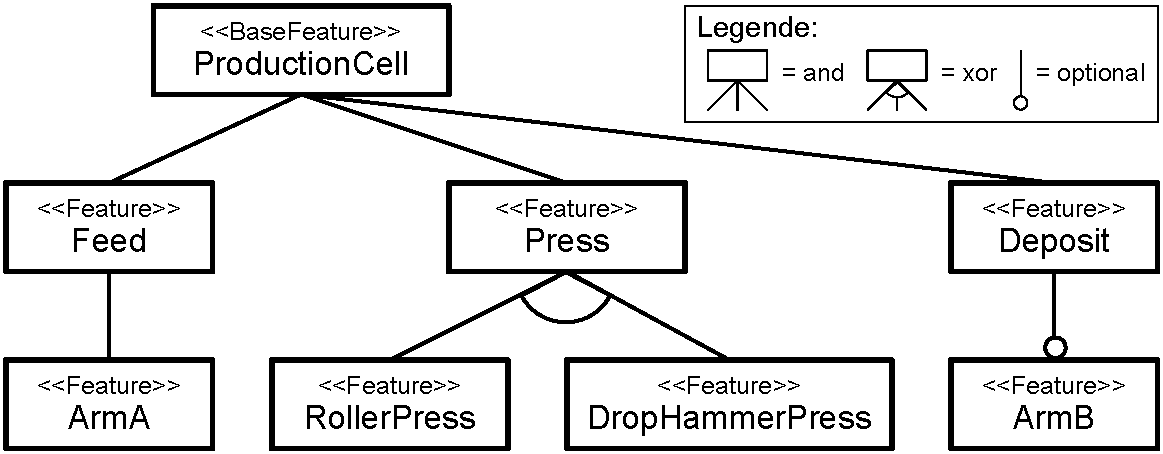
\includegraphics[scale=\stdScaleFactor]
 {contents/figures/feature-diagram-productioncell-example.pdf}
 \caption{Das Featurediagramm eines Produktionsroboters}
 \label{fig:feature-diagram-productioncell-example}
\end{figure}

Achten Sie darauf, dass jede ung gut lesbar ist und nicht den Rand des Textbereichs überschreitet. Eine Abbildung muss immer im Text referenziert und beschrieben werden. Was sieht der Leser? Was bedeuten zum Beispiel verschiedene Pfeile? Eine Legende in der Grafik (wie in Abb.\,\ref{fig:feature-diagram-productioncell-example}) ist nicht zwingend notwendig, kann die Grafik aber besser verständlich machen. Sie können das Wort "`Abbildung"' im Text mit "`Abb."' abkürzen. An Satzanfängen sieht die ausgeschriebene Variante allerdings schöner aus.

\paragraph{\textit{Empfehlungen}:}

\begin{itemize}
    \item Positionieren Sie Abbildungen möglichst nah an der Stelle, wo sie im Text referenziert und erklärt werden. In \LaTeX{} benutzen Sie für das Einbinden von Abbildungen mittels der \texttt{figure}-Umgebung am besten den Parameter \texttt{[h]}: 
    
    \begin{verbatim}
        \begin{figure}[h] ... \end{figure}
    \end{verbatim}
    
    \item In Abbildungen nutzen Sie besser serifenlose Schriften, wie zum Beispiel Arial. Die Schrift in Grafiken sollte etwas kleiner als der Fließtext sein, ca. 60\%-90\%, aber nicht weniger als 50\%, da die Schrift sonst zu klein und nicht mehr lesbar wird. Außerdem sollten die Schriften in Abbildungen konsistent in der Größe sein. Verwenden Sie daher eine einheitliche Schrift und Schriftgröße in den Abbildungen und einen einheitlichen Skalierungsfaktor für Abbildungen im Text.
\end{itemize}



\section{Schreibstil}

\subsection{Aktiv und Passiv, Verwendung von \textit{ich}}

Der wissenschaftliche Schreibstil hat sich in den letzten Jahren gewandelt. Früher waren lange, verschachtelte Sätzen ein Zeichen von Wissenschaftlichkeit und Autoren schrieben in passiver Form, um die Personalpronomen \enquote{wir} und \enquote{ich} zu vermeiden -- \enquote{wir} und \enquote{ich} klinge \enquote{weniger objektiv}, so oft die Begründung.

Das hat sich geändert. Heute ist es in technischen Bereichen, auch durch den angelsächsischen Einfluss, ein Zeichen guten Ausdrucks, möglichst im Aktiv zu schreiben. Passive Sätze wirken distanziert und sind oft komplizierter als aktive Sätze. Daher raten wir zur aktiven Sprache. 

Wenn Sie in der Arbeit Ihr eigenes Vorgehen, Abwägungen oder Entscheidungen beschreiben, sollten Sie insbesondere die Personalpronomen \enquote{wir} und \enquote{ich} verwenden. Diese Ausführungen sind inhärent \textit{subjektiv} und sollten auch nicht den falschen Anschein von Objektivität erwecken.

In wissenschaftlichen Veröffentlichungen im technischen Bereich wird oft \enquote{wir} (oder engl. \enquote{we}) verwendet, ein \enquote{ich} findet man seltener. Das liegt allerdings daran, dass wissenschaftliche Arbeiten meist von mehr als einer Person durchgeführt und veröffentlicht werden. Selbst wenn eine Veröffentlichung nur einen Autor hat, schreibt dieser Autor meist \enquote{wir}, weil die Arbeit selten von dem Autor allein stammt, sondern auch eine Forschergruppe dahinter steht.

Bei studentischen Arbeiten ist das anders, da diese eigenständige Studienleistungen sind, die Sie auch wirklich allein bearbeiten müssen. Zudem müssen Sie in der schriftlichen Darstellung deutlich machen, welche Ergebnisse Sie persönlich produziert haben und welche Beiträge anderen zuzuschreiben sind, zum Beispiel Kollegen im Partnerunternehmen.

Nehmen wir den passiven Satz \enquote{Es wurde eine Problemanalyse durchgeführt und Anforderungen wurden abgeleitet.} -- Wer hat denn die Problemanalyse durchgeführt und Anforderungen abgeleitet? Der Autor des Textes? Oder bezieht sich der Autor auf Vorarbeiten von Kollegen? Das wird in dieser Formulierung nicht klar! 

Schreiben Sie besser \enquote{Ich habe eine Problemanalyse durchgeführt und Anforderungen abgeleitet}. Haben vielleicht Kollegen dabei geholfen? Welchen Anteil hatte dabei der Kollege? Machen Sie dies explizit deutlich und schreiben Sie zum Beispiel: \enquote{Ich habe eine Problemanalyse durchgeführt und eine erste Liste von Anforderungen abgeleitet. Diese Liste habe ich daraufhin zusammen mit Kollegen der Abteilung konkretisiert und priorisiert.} Nun wird deutlich, welchen Beitrag Sie geleistet haben! Ihre Prüfer können Ihre Leistung nun eindeutiger beurteilen.

Gehen Sie jedoch sparsam mit \enquote{ich} oder \enquote{wir} um und beschränken Sie deren Verwendung auf Stellen, an denen Sie Ihr eigenes Vorgehen, Abwägungen oder Entscheidungen beschreiben -- eine Praxis- oder Abschlussarbeit ist kein Tagebuch und keine Erzählung aus der Ich-Perspektive!

Die passive Schreibweise müssen Sie natürlich nicht vollständig verbannen. Dort wo eine Handlung im Vordergrund steht und nicht der Handelnde, können Sie das Passiv verwenden. Beispiel: \enquote{Bei der testgetriebenen Entwicklung werden Anforderungen bereits in Testfälle überführt, bevor die entsprechende Softwarefunktionen entwickelt werden.} Jedoch kann es auch hier hilfreich sein, zu erklären, welche Personen oder Rollen am Geschehen beteiligt sind -- gerade wenn es um Arbeitsprozesse geht. Wer schreibt die Tests? Ein Tester? Der Entwickler selbst? Vielleicht ist es doch besser zu schreiben \enquote{Bei der testgetriebenen Entwicklung überführt der Entwickler oder die Entwicklerin die Anforderungen in Testfälle, schon bevor er/sie die entsprechenden Softwarefunktionen entwickelt.}

\subsection{Wortwahl}

Vermeiden Sie lange, verschachtelte Sätze sowie überflüssige Worte und vage Formulierungen.

\paragraph{\textit{Empfehlung}:}
Es gibt viele Quellen, auch online, mit Tipps zum Schreiben. Recherchieren Sie und reflektieren Sie über Ihre Ausdrucksweise.


\section{Arbeit mit Quellen}
\label{sec:arbeit-mit-quellen}

Bei der Erklärung von Grundlagen, Problemstellungen, Lösungsansätzen, verwandten Arbeiten oder zur Unterstützung von Argumenten sollten Sie auf geeignete Quellen hinweisen. Hier Beispiele für Referenzen auf Quellen~\cite{Greenyer2007,Greenyer2013}, welche im Quellverzeichnis aufgelistet sind. 
Sie können numerische oder auch alphabetische Verweisstile verwenden (siehe auch \url{https://www.overleaf.com/learn/latex/Articles/Getting_started_with_BibLaTeX}). Verwenden Sie für Zitate keine Fußnoten, wie dies in anderen Bereichen üblich ist.

Achten Sie beim Quellenverzeichnis darauf, dass dort alle Quellen aufgelistet sind, die Sie im Text zitiert haben (und auch nur diese!).

\paragraph{\textit{Empfehlung}:}
Wenn Sie mit \LaTeX{} arbeiten, verwenden Sie \textit{Bibtex}. Für mehrere Quellverzeichnisse verwenden Sie \textit{Multibib} (\url{https://www.overleaf.com/learn/latex/Multibib}).

Sie können die Quellen in ein Quellverzeichnis sortieren oder mehrere Quellverzeichnisse nach Publikationstyp getrennt verwenden. Dieses bietet sich an um wissenschaftliche Quellen und nicht-wissenschaftliche Quellen eindeutig zu trennen, ist aber optional.

\subsection{Korrekt zitieren}

Achten Sie auf die Vollständigkeit der Quellenangaben. Wenn Sie \LaTeX{} und Bibtex verwenden, werden die Angaben meist automatisch in der richtigen Reihenfolge generiert. Sie können oft auf den Webseiten der Verlage fertige Bibtex-Einträgen zu Quellen finden. Viele Verlage, wie zum Beispiel Springer, ACM, IEEE, etc. (s. Links unten), bieten für ihre Veröffentlichungen meist vollständige und korrekte Bibtex-Einträge zum Download an. Zur Verwaltung von Quellen können Sie Werkzeuge wie JabRef (\url{https://www.jabref.org/}) nutzen, welches auch Funktionen für die Suche und den automatischen Import von Bibtex-Einträgen bietet. Wenn Sie irgendwo anders im Internet Bibtex-Einträgen finden, vertrauen Sie nicht darauf, dass diese vollständig und richtig sind. Prüfen Sie in jedem Fall die finale Darstellung Ihre Quellenangaben im Dokument. 

Erforderliche Angaben zu den Quellen, je nach Art der Quelle, sind im Folgenden beschrieben:

\begin{itemize}
    
    \item \textbf{Monographien und Lehrbücher} (Bibtex-Typ \texttt{@book}): 
    Es erscheinen zuerst die Autoren mit erst Nachname, dann Vorname. Es folgt ein Punkt oder Doppelpunkt (aber: konsistent bleiben), dann der Titel der Publikation, Verlag und optional Erscheinungsort(e). Danach folgt die Zahl der Ausgabe, falls nicht die erste. Zuletzt wird das Jahr der Veröffentlichung genannt. Beispiel: \cite{Sutton2018}
    
    \item \textbf{Fachartikel in Zeitschriften} (Bibtex-Typ \texttt{@article}): 
    Wieder erscheinen zuerst die Autoren, dann der Titel des Artikels. Es folgt der Zeitschriftentitel sowie die Heftnummer (number),  Band (volume), Seitenbereich und Jahresangabe. Beispiel: \cite{Greenyer2013}
    
    \item \textbf{Konferenzbeiträge} (Bibtex-Typ \texttt{@inproceedings}): 
    Wieder erscheinen zuerst die Autoren, dann der Titel des Artikels. Es folgt die Nennung des Konferenzbandes, wobei, wenn bekannt, die Herausgeber (Editoren) des Konferenzbandes vorangestellt werden.
    Darauf folgt optional Serie, Heftnummer und Band, und schließlich Seitenbereich und Jahresangabe. Beispiel: \cite{Greenyer2007}
    
    \item \textbf{Internetquellen} (Bibtex-Typ \texttt{@misc}): Sie können auch Online-Artikel, Wikipedia-Einträge, API-Referenzen, Podcasts, Blog-Einträge, Videos, Social-Media-Beiträge oder andere Quellen im Internet zitieren.
    Geben Sie auch hier erst, soweit vorhanden, die Namen der Autoren an, dann den Titel, gegebenenfalls den Namen eines Online-Magazins, ein Veröffentlichungsdatum, dann die URL der Quelle und das Zugriffsdatum. Beispiel: \cite{Gebhard2021}
    
    \item Es gibt weitere Arten von Quellen, wie Buchkapitel, Masterarbeiten, Doktorarbeiten, technische Berichte oder Standards. Auch hier werden zuerst Autoren und dann der Titel genannt. Weiter Angaben variieren. Recherchieren Sie nach einer gängigen Zitierweise und korrekter Nutzung von Eintrags-Typen in Bibtex. Hier ein Beispiel für den Verweis auf einen Standard: \cite{UML251}.
\end{itemize}


\subsection{Zitate im Text}

Wenn Sie Textstellen wörtlich oder wörtlich übersetzt aus anderen Quellen wiedergeben, müssen Sie diese Textbereiche \textbf{eindeutig durch Anführungszeichen} kennzeichnen.
Hier ein Beispiel für ein wörtliches, übersetztes Zitat: \enquote{Heute werden oft nicht nur einzelne Softwareprodukte entwickelt, sondern ganze Produktlinien, also es müssen viele Varianten eines Produkts entwickelt werden.} \cite[Seite~1]{Greenyer2013}.

\textbf{\textit{Empfehlung:}} Gehen Sie sparsam mit übernommenen Textpassagen um. Wörtlich übernommene Textpassagen sollen Ihre eigenen Inhalte ergänzen und unterstützen, diese nicht ersetzen. Wenn ein Grundlagen-Kapitel eine Aneinanderreihung kopierter Passagen aus fremden Quellen ist, werden die Inhalte nicht als Ihre kreative Leistung anerkannt.

Allgemein sollte eine Referenz nicht als Textelement genutzt werden\footnote{Dasselbe gilt für Fußnoten. Fußnoten sollten übrigens nur in Ausnahmefällen eingesetzt werden, wenn eine zusätzliche Anmerkung nur sehr schwer im Haupttext erwähnt werden kann, ohne den Textfluss, wie zum Beispiel eine Argumentationskette, zu unterbrechen. Eine gute Arbeit kommt sehr gut ohne Fußnoten aus: Sind Anmerkungen wichtig, sollten sie in den Haupttext integriert werden. Sind sie nicht wichtig, warum sollten sie dann in der Arbeit erwähnt werden? Oder fanden Sie es jetzt gut, vom Lesefluss abgelenkt zu werden, nur um hier etwas im Kleingedruckten zu lesen und gleich wieder die Textstellen suchen zu müssen, wo Sie weiterlesen wollten?}. Also nicht so: Eine effiziente Methode zur Konsistenzanalyse wird in~\cite{Cordy2012} beschrieben. Sondern so: Eine effiziente Methode zur Konsistenzanalyse wird beschrieben von Cordy et al.\,\cite{Cordy2012}. Der Text sollte also auch lesbar sein, wenn die Verweise entfernt würden. Die Abkürzung \textit{et al.} bedeutet übrigens \enquote{et alii}, auf Deutsch \enquote{und andere}; diese Ausdruck wird in wissenschaftlichen Schriften gerne verwenden, wenn von mehr als zwei Autoren die Rede ist, um diese nicht alle aufzählen zu müssen.

Wenn Sie zitieren, sollten sie, zumindest in einer Bachelor- oder Master-Thesis, möglichst wissenschaftliche Quellen zitieren. Das sind Papiere von Workshops und Konferenzen, sowie Dissertationen, Fachbücher oder Artikel in Fachjournalen. Diese Quellen sind meist vertrauenswürdig, da sie einen Begutachtungsprozess durchlaufen. Technische Berichte werden typischerweise nicht begutachtet, sind aber meist vertrauenswürdig wenn Sie von Wissenschaftlern verfasst sind, die weitere, begutachtete Papiere zu demselben Themenbereich veröffentlicht haben.

Bei der Recherche sind diese Internetseiten hilfreich:
\begin{itemize}
  \item \url{http://scholar.google.com}
  \item \url{http://academic.research.microsoft.com/}
  \item \url{http://ieeexplore.ieee.org/}
  \item \url{http://dl.acm.org/dl.cfm}
  \item \url{http://www.springerlink.com/}
  \item \url{https://www.springerprofessional.de/} (die FHDW hat hier Zugänge -- sprechen Sie Ihren Erstprüfer darauf an.)
  \item \url{http://liinwww.ira.uka.de/bibliography/}
  \item \url{http://www.informatik.uni-trier.de/~ley/db/}
\end{itemize}

Verweise auf Internetquellen wie zum Beispiel Artikel von Onlinemagazinen oder Wikipediaartikel sind auch möglich, sollten aber nur verwendet werden, wenn es keine passende wissenschaftliche Quelle gibt. 
In Praxisarbeiten kann der Großteil der Quellverweise aus Internetquellen kommen, weil es sich dort oft um eine sehr praxisnahe Fragestellung handelt. Bei einer Bachelor-Thesis oder Master-Thesis sollten jedoch auch, wenn nicht gar hauptsächlich, wissenschaftlicher Quellen genannt werden (siehe auch Kapitel~\ref{chap:struktur-und-inhalt}).


\section{Plagiarismus}

Eine wissenschaftliche Arbeit steht immer in Zusammenhang mit anderen Arbeiten. Verweise auf Quellen sind in wissenschaftlichen Arbeiten daher unerlässlich und förderlich für das Verständnis. Wenn Sie Sätze oder Textpassagen \textbf{wörtlich oder sinngemäß} (zum Beispiel übersetzt ins Deutsche) aus anderen Quellen in Ihre Arbeit übernehmen, dann müssen diese Stellen explizit gekennzeichnet werden (mit Anführungszeichen, siehe oben). \textbf{Es muss eindeutig erkennbar sein, welche Teile Ihrer Arbeit Ihren eigenen kreativen Beitrag darstellen, und welche Teile Sie aus anderen Quellen übernommen haben.} Auch wenn Sie Bilder aus Quellen andere Urheber übernehmen, müssen Sie dies explizit kenntlich machen (zum Beispiel \enquote{Grafik entnommen aus\ldots}). Dasselbe gilt auch für Sourcecode, Skripte oder Datensätze, die Sie aus anderen Quellen übernehmen.

Wenn Sie Bilder, Code oder längere Textpassagen in Ihre Arbeit übernehmen, erkundigen Sie sich, ob das diese Inhalte \textbf{urheberrechtlich geschützt} sind. In gewissem Umfang dürfen Sie diese Inhalte in Ihrer Arbeit \enquote{zum Zweck der nicht kommerziellen wissenschaftlichen Forschung} wiederverwenden und vervielfältigen, siehe §60c UrhG. Diese Ausnahme gilt allerdings nicht, wenn Sie Bilder rein zur visuellen Dekoration verwenden.

Auch \textbf{Beispiele}, die inhaltlich aus Quellen übernommen werden, müssen gekennzeichnet sein, selbst wenn Sie neue Grafiken anfertigen (die dann aber wieder sinngemäß aus der Quelle übernommen sind). Sind die Erklärungen zu dem Beispiel Ihre eigenen Worte, reicht eine Angabe wie zum Beispiel "`Das in dieser Arbeit / im folgenden Abschnitt erklärte Beispiel ist entnommen aus Cordy et al.~\cite{Cordy2012}\ldots"'. Erweitern Sie Beispiele aus Quellen, sollten die übernommenen Teile des Beispiels und Ihre Erweiterungen klar genannt werden.

Für die Bewertung zählt Ihr eigener Beitrag! Wenn Sie fremde Inhalte übernehmen, werden also nicht die fremden Inhalte bewertet, sondern Ihre eigenen Erweiterungen, Schlussfolgerungen, Argumentationen oder Verknüpfungen.

Wenn Sie fremde Inhalte vorsätzlich oder fahrlässig als Ihre eigenen Ausgeben, führt dies \textbf{mindestens zum Nichtbestehen} Ihrer Arbeit!